\documentclass[12pt,a4paper]{article}
\usepackage[utf8]{vietnam}
\usepackage{amsmath,amssymb}
\usepackage{tabularx}
\usepackage{tikz}
\usetikzlibrary{calc,angles,quotes,arrows.meta}
\usepackage{xcolor}
\usepackage{enumitem}
\usepackage{fancyhdr}
\usepackage[top=1.2cm, bottom=1.2cm, left=1.5cm, right=1.5cm]{geometry}
\usepackage[dethi]{ex_test}
\SAOPTN{widthSA=2.6,heightSA=0.62}

\setlength{\headheight}{15pt}
\setlength{\parskip}{0pt}

% Dòng kẻ chấm mờ chuẩn viết tay
\newcommand{\dongke}[1]{%
  \begingroup%
  \setlength{\parskip}{0pt}%
  \baselineskip=18.5pt%
  \vspace{1.0mm}%
  \foreach \i in {1,...,#1}{%
    \noindent{\color{gray!60}\dotfill}\par%
  }%
  \vspace{0.6mm}%
  \endgroup%
}

\pagestyle{fancy}
\fancyhf{}
\rhead{\textit{Môn Toán 7 -- Đề số 2}}
\lhead{\textit{Bộ đề ôn tập Giữa học kì I}}
\cfoot{\thepage}

\begin{document}

% --- KHUNG TIÊU ĐỀ ĐỀ THI ---
\noindent
\begin{tabularx}{\linewidth}{X r}
\textbf{TRƯỜNG THCS: \dotfill} & \textbf{ĐỀ KIỂM TRA ĐỊNH KỲ GIỮA HỌC KỲ I} \\
\textbf{Họ và tên: \dotfill} & \textbf{NĂM HỌC 2026 -- 2027} \\
\textbf{Lớp: \dotfill \quad SBD: \dotfill} & \textbf{Môn: TOÁN 7} \\
& \textit{Thời gian làm bài: 90 phút (không kể thời gian phát đề)}
\end{tabularx}

\vspace{1.5mm}
\noindent
\begin{tabularx}{\linewidth}{|p{3.5cm}|X|}
\hline
\centering\textbf{Điểm số} & \centering\textbf{Lời nhận xét của thầy cô giáo} \tabularnewline
\rule{0pt}{1.6cm} & \\
\hline
\end{tabularx}

\vspace{2.5mm}
\begin{center}
\textbf{\large ĐỀ SỐ 2}
\end{center}

\noindent\textbf{\large PHẦN I. CÂU TRẮC NGHIỆM NHIỀU PHƯƠNG ÁN LỰA CHỌN (3,0 điểm)}

\textit{Thí sinh trả lời từ câu 1 đến câu 12. Mỗi câu hỏi chỉ chọn một phương án đúng nhất và ghi vào bảng đáp án.}

\vspace{1mm}
\begin{ex}
Số nào sau đây là số hữu tỉ?
\choice
{$\sqrt{5}$}
{$\sqrt{2}$}
{$\sqrt{3}$}
{\True $\sqrt{4}$}
\end{ex}

\begin{ex}
Số đối của $-\dfrac{2}{3}$ là:
\choice
{\True $\dfrac{2}{3}$}
{$\dfrac{3}{2}$}
{$-\dfrac{3}{2}$}
{$-\dfrac{2}{3}$}
\end{ex}

\begin{ex}
Giá trị của $|-3|$ bằng
\choice
{$-3$}
{\True $3$}
{$\dfrac{1}{3}$}
{$-\dfrac{1}{3}$}
\end{ex}

\begin{ex}
Qua một điểm $M$ nằm ngoài đường thẳng $a$, kẻ được bao nhiêu đường thẳng song song với đường thẳng $a$?
\choice
{Có vô số đường thẳng}
{Không có đường thẳng nào}
{Có hai đường thẳng}
{\True Chỉ có một đường thẳng}
\end{ex}

\begin{ex}
Nếu hai đường thẳng phân biệt cùng song song với một đường thẳng thứ ba, thì:
\choice
{Chúng cắt nhau}
{Chúng trùng nhau}
{\True Chúng cũng song song với nhau}
{Chúng vuông góc với nhau}
\end{ex}

\begin{ex}
Trong các số sau, số nào là số hữu tỉ âm?
\choice
{$-\dfrac{0}{2}$}
{$\dfrac{-2}{-1}$}
{\True $-\dfrac{1}{2}$}
{$-\dfrac{-2}{3}$}
\end{ex}

\begin{ex}
Khối Rubik $4 \times 4$ có hình dạng là hình lập phương có cạnh $6\text{ cm}$. Thể tích của khối Rubik là:
\choice
{$216\text{ cm}^2$}
{$144\text{ cm}^3$}
{$144\text{ cm}^2$}
{\True $216\text{ cm}^3$}
\end{ex}

\begin{ex}
Các mặt của hình lập phương là:
\choice
{\True Hình vuông}
{Tam giác đều}
{Hình chữ nhật}
{Hình thoi}
\end{ex}

\begin{ex}
Điền cụm từ thích hợp vào chỗ trống để được khẳng định đúng: “Qua một điểm ở ngoài một đường thẳng, \dots đường thẳng song song với đường thẳng đó”.
\choice
{\True Chỉ có một}
{Có vô số}
{Có hai}
{Không có}
\end{ex}

\begin{ex}
Cho các số sau: $\dfrac{5}{-4}; 3\dfrac{2}{5}; \dfrac{-2}{7}; \dfrac{0}{3}; \dfrac{3}{0}; -\dfrac{-8}{8}; 0{,}625$. Hãy cho biết số nào không phải là số hữu tỉ?
\choice
{\True $\dfrac{3}{0}$}
{$0{,}625$}
{$-\dfrac{2}{7}$}
{$3\dfrac{2}{5}$}
\end{ex}

\begin{ex}
Cho biểu thức $-\left(1-\dfrac{1}{2}\right)+\left(2+\dfrac{1}{3}\right)-\left(3-\dfrac{1}{2}+\dfrac{1}{3}\right)$. Khi bỏ dấu ngoặc, ta được biểu thức nào sau đây:
\choice
{$-1+\dfrac{1}{2}+2+\dfrac{1}{3}-3-\dfrac{1}{2}+\dfrac{1}{3}$}
{\True $-1+\dfrac{1}{2}+2+\dfrac{1}{3}-3+\dfrac{1}{2}-\dfrac{1}{3}$}
{$-1+\dfrac{1}{2}+2+\dfrac{1}{3}+3-\dfrac{1}{2}-\dfrac{1}{3}$}
{$-1+\dfrac{1}{2}+2+\dfrac{1}{3}-3+\dfrac{1}{2}-\dfrac{1}{3}$}
\end{ex}

\begin{ex}
Số đối của $-\dfrac{1}{3}$ là:
\choice
{\True $\dfrac{1}{3}$}
{$3$}
{$-\dfrac{1}{3}$}
{$-\dfrac{-1}{3}$}
\end{ex}


\vspace{1mm}
\noindent\textbf{BẢNG TRẢ LỜI TRẮC NGHIỆM PHẦN I:}
\begin{center}
\begin{tabular}{|c|c|c|c|c|c|c|c|c|c|c|c|c|}
\hline
\textbf{Câu} & \textbf{1} & \textbf{2} & \textbf{3} & \textbf{4} & \textbf{5} & \textbf{6} & \textbf{7} & \textbf{8} & \textbf{9} & \textbf{10} & \textbf{11} & \textbf{12} \\
\hline
\textbf{Chọn} & \rule{0pt}{0.65cm} & & & & & & & & & & & \\
\hline
\end{tabular}
\end{center}
\vspace{2mm}

\setcounter{ex}{0}
\noindent\textbf{\large PHẦN II. CÂU TRẮC NGHIỆM ĐÚNG SAI (2,0 điểm)}

\textit{Thí sinh trả lời câu 1 và câu 2. Trong mỗi ý a), b), c), d) ở mỗi câu, thí sinh chọn đúng hoặc sai.}

\vspace{1mm}
\begin{ex}
\immini{
Quan sát hình vẽ, hai đường thẳng $a$ và $b$ cắt nhau tại điểm $O$ tạo thành bốn góc $\widehat{O_1}, \widehat{O_2}, \widehat{O_3}, \widehat{O_4}$. Xét tính đúng sai của các mệnh đề sau:
\choiceTF
{\True Góc $\widehat{O_1}$ và góc $\widehat{O_3}$ là hai góc đối đỉnh}
{Góc $\widehat{O_2}$ và góc $\widehat{O_4}$ là hai góc kề bù}
{\True Tổng số đo của góc $\widehat{O_1}$ và góc $\widehat{O_2}$ bằng $180^\circ$}
{\True Nếu số đo góc $\widehat{O_1}$ bằng $50^\circ$ thì số đo góc $\widehat{O_2}$ bằng $130^\circ$}
}{
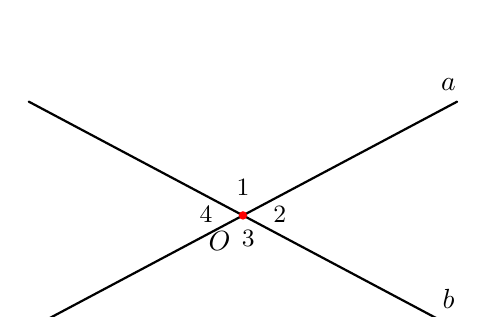
\begin{tikzpicture}[scale=0.85, line cap=round, line join=round]
  \coordinate (O) at (0,0);
  % Duong a nghieng 28 do
  \draw[thick] (-3.2,-1.7) -- (3.2,1.7) node[above=2pt, pos=0.98] {$a$};
  % Duong b nghieng -28 do
  \draw[thick] (-3.2,1.7) -- (3.2,-1.7) node[above=2pt, pos=0.98] {$b$};

  % Giao diem O
  \fill[red] (O) circle (1.8pt);
  \node[font=\normalsize] at (-0.35, -0.38) {$O$};

  % 4 goc tai O
  \node[font=\small] at (0, 0.42) {$1$};
  \node[font=\small] at (0.55, 0.02) {$2$};
  \node[font=\small] at (0.08, -0.35) {$3$};
  \node[font=\small] at (-0.55, 0.02) {$4$};
\end{tikzpicture}
}
\end{ex}

\begin{ex}
Hai bạn Việt và Nam mỗi người mang $30\,000$ đồng đi đến cửa hàng mua một cuốn truyện. Cuốn truyện Conan của Việt mua có giá niêm yết là $20{,}8$ nghìn đồng và được giảm giá $5\%$. Cuốn truyện Doraemon của Nam mua có giá $21{,}2$ nghìn đồng và được giảm giá $6\%$. Do đó, Việt và Nam định góp số tiền thừa mua thêm một cuốn truyện nữa. Xét tính đúng sai của các mệnh đề sau:
\choiceTF
{\True Cuốn truyện Việt mua được giảm $1\,040$ đồng}
{\True Cuốn truyện Nam mua được giảm $1\,272$ đồng}
{Sau khi giảm giá, bạn Nam cần trả ít tiền hơn bạn Việt}
{Tổng số tiền còn lại của hai bạn không đủ mua cuốn truyện nào}
\end{ex}


\noindent\textbf{BẢNG TRẢ LỜI PHẦN II:}
\begin{center}
\begin{tabular}{|c|c|c|c|c||c|c|c|c|c|}
\hline
\textbf{Câu 1} & \textbf{a)} & \textbf{b)} & \textbf{c)} & \textbf{d)} & \textbf{Câu 2} & \textbf{a)} & \textbf{b)} & \textbf{c)} & \textbf{d)} \\
\hline
\textbf{Đ/S} & \rule{0pt}{0.6cm} & & & & \textbf{Đ/S} & & & & \\
\hline
\end{tabular}
\end{center}
\vspace{2mm}

\setcounter{ex}{0}
\noindent\textbf{\large PHẦN III. CÂU HỎI TRẢ LỜI NGẮN (1,0 điểm)}

\textit{Thí sinh trả lời câu 1 và câu 2. Điền kết quả vào ô trống.}

\vspace{1mm}
\begin{ex}
Quan sát trục số sau rồi cho biết: Điểm $A$ và điểm $B$ biểu diễn số hữu tỉ nào?
\begin{center}
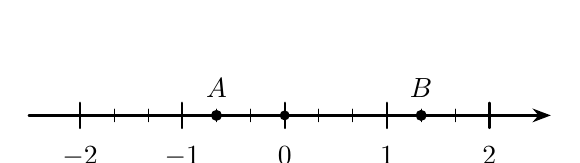
\begin{tikzpicture}[x=1.3cm, y=1cm, line cap=round, line join=round, >=Stealth]
  % Truc so
  \draw[thick, ->] (-2.5,0) -- (2.6,0);

  % Cac vach chia phan 3
  \foreach \i in {-6,-5,...,6}{
    \draw (\i/3, 0.08) -- (\i/3, -0.08);
  }

  % Cac vach so nguyen chinh va nhan so
  \foreach \x in {-2,-1,0,1,2}{
    \draw[thick] (\x, 0.16) -- (\x, -0.16) node[below=3pt] {$\x$};
  }

  % Diem O cham den tai goc
  \fill (0,0) circle (1.8pt);

  % Diem A tai -2/3
  \fill (-2/3, 0) circle (2.0pt);
  \node[above=3pt, font=\bfseries] at (-2/3, 0) {$A$};

  % Diem B tai 4/3 = 1 1/3
  \fill (4/3, 0) circle (2.0pt);
  \node[above=3pt, font=\bfseries] at (4/3, 0) {$B$};
\end{tikzpicture}
\end{center}
\hfill\shortans{$A = -\dfrac{2}{3}; B = \dfrac{4}{3}$}
\end{ex}

\begin{ex}
Tìm số thực $x$, biết: $\left(x-\dfrac{1}{2}\right)^3 + \dfrac{5}{8} = -15$ (kết quả ghi dưới dạng số thập phân). \shortans{-2}
\end{ex}


\setcounter{ex}{0}
\noindent\textbf{\large PHẦN IV. TỰ LUẬN (4,0 điểm)}

\textit{Thí sinh trình bày chi tiết lời giải vào giấy làm bài.}

\vspace{1mm}
\begin{ex}
Thực hiện phép tính (Tính nhanh nếu có thể):
\begin{enumerate}[label=\textbf{\alph*)}, leftmargin=0.8cm, itemsep=1pt]
\item $\dfrac{9}{8} - \dfrac{1}{8} : \dfrac{3}{4}$
\item $\dfrac{23}{25} - \dfrac{19}{43} + \dfrac{27}{25} - \dfrac{24}{43}$
\item $-\dfrac{2}{5} \cdot \dfrac{17}{9} - \dfrac{2}{5} \cdot \dfrac{8}{9} + \dfrac{16}{5}$
\end{enumerate}
\end{ex}
\vspace{1.5mm}

\begin{ex}
Tìm $x$, biết:
\begin{enumerate}[label=\textbf{\alph*)}, leftmargin=0.8cm, itemsep=1pt]
\item $x - 2\dfrac{1}{3} = \dfrac{1}{6}$
\item $x^2 = \dfrac{1}{16}$
\end{enumerate}
\end{ex}
\vspace{1.5mm}

\begin{ex}
\immini{
Cho hình vẽ bên:
\begin{enumerate}[label=\textbf{\alph*)}, leftmargin=0.8cm, itemsep=1pt]
\item Giải thích tại sao $yy' \parallel zz'$?
\item Tính số đo góc $\widehat{ABz}$?
\end{enumerate}
}{
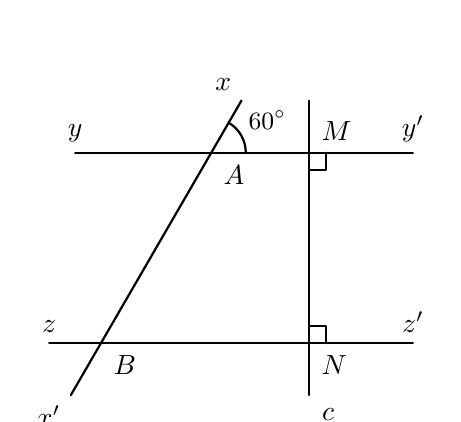
\begin{tikzpicture}[scale=1.1, line cap=round, line join=round]
  \coordinate (B) at (0,0);
  \coordinate (N) at (2.4,0);
  \coordinate (A) at (1.27,2.2);
  \coordinate (M) at (2.4,2.2);

  % Duong vuong goc c qua M va N
  \draw[thick] (2.4, 2.8) -- (2.4, -0.6) node[below right=1pt] {$c$};

  % Duong yy'
  \draw[thick] (-0.3, 2.2) node[above] {$y$} -- (3.6, 2.2) node[above] {$y'$};

  % Duong zz'
  \draw[thick] (-0.6, 0) node[above] {$z$} -- (3.6, 0) node[above] {$z'$};

  % Cat tuyen xx'
  \draw[thick] (-0.35, -0.6) node[below left] {$x'$} -- (1.62, 2.8) node[above left] {$x$};

  % Ký hiệu góc vuông tại M và N
  \draw[thick] (2.4, 2.0) -- (2.6, 2.0) -- (2.6, 2.2);
  \draw[thick] (2.4, 0.2) -- (2.6, 0.2) -- (2.6, 0);

  % Cung goc 60 do tai A
  \draw[thick] (A) ++(0:0.4) arc[start angle=0, end angle=60, radius=0.4];
  \node[font=\small] at ($(A)+(30:0.75)$) {$60^\circ$};

  % Nhan cac dinh
  \node[below right=1pt] at (A) {$A$};
  \node[above right=1pt] at (M) {$M$};
  \node[below right=1pt] at (B) {$B$};
  \node[below right=1pt] at (N) {$N$};
\end{tikzpicture}
}
\end{ex}
\vspace{1.5mm}

\begin{ex}
Cho $M = \dfrac{1}{2} + \dfrac{1}{3^2} + \dfrac{1}{3^4} + \dfrac{1}{3^6} + \dots + \dfrac{1}{3^{802}}$. Chứng minh rằng: $M < \dfrac{3}{8}$.
\end{ex}
\vspace{1.5mm}


\begin{center}
\rule{4cm}{0.4pt}\\
\textit{--- HẾT ---}
\end{center}
\end{document}
